\chapter{Конструкторский раздел}
\label{cha:design}

В данном разделе рассматриваются реализуемые методы, алгоритмы. Приводится
схема приложения и диаграмма классов.

\section{Метод конструктивной сплошной геометрии}
Данный метод делится на несколько алгоритмов, рассматриваемых ниже.

% \subsection{Знаковая функция расстояния и алгоритмы композиции тел}
Знаковая функция расстояния (англ. $SDF$) может быть использована для получения кратчайшего 
расстояния от точки до поверхности тела, причём отрицательный знак соответствует положению точки внутри тела.
Ниже рассматриваются $SDF$ для сферы и куба.

Для получения $SDF$ сферы необходимо знать расстояние до её центра от заданной точки (см. формулу \ref{eq:center_of_sphere})
и длину радиуса.
\begin{equation} \label{eq:center_of_sphere}
  length(x,y,z) = \sqrt{(x - x_0)^2 + (y - y_0)^2 + (z - z_0)^2}
\end{equation}
где $C(x_0, y_0, z_0)$ - центр координат,
$p(x, y, z)$ - рассматриваемая точка.  

Подставляя формулу \ref{eq:center_of_sphere} в формулу расстояния \ref{eq:sdf_sphere} можно получить
$SDF$ сферы.
\begin{equation} \label{eq:sdf_sphere}
  dist = length(x, y, z) - r
\end{equation}
Для куба необходимо учесть 3 расположения точки относительно граней и 
получить формулу \ref{eq:sdf_box} $SDF$ куба.
% объединить всё в одну формулу (см. \ref{eq:sdf_box}), получив SDF куба.
\begin{equation} \label{eq:sdf_box}
  \begin{cases}
    q = abs(p) - r  \\
    dist = length(max(q, 0.0)) + min(max(q.x, max(q.y,q.z)), 0.0)
  \end{cases}
\end{equation}
где $p(x, y, z)$ - рассматриваемая точка,
$q(x, y, z)$ - координаты точки за вычетом радиуса,
$dist$ - искомое расстояние с учётом двух расположений точки относительно граней и угла.

Данные $SDF$ позволяют эффективно использовать алгоритм маршировки лучей, так как луч двигается
к рассматриваемому объекту с максимальным шагом, который не приведёт к пропуску лицевой грани объекта.

$SDF$ используется в моделировании тел $CSG$.
Алгоритмы композиции необходимо использовать, чтобы связать методы создания тел и визуализации

При пересечении двух тел (см. формулу \ref{eq:sdf_intersect}) луч должен пересечься с тем, которое дальше от камеры, следовательно,
необходимо выбрать $SDF$ с наибольшим значением.
\begin{equation} \label{eq:sdf_intersect}
  intersection(sdf1, sdf2, x, y, z) = max(sdf1(x, y, z), sdf2(x, y, z))
\end{equation}
где $sdf1$, $sdf2$ - функции, возвращающие расстояние до точки с координатами $x$, $y$, $z$.

Для объединения (см. формулу \ref{eq:sdf_union}) тел луч должен пересечься с ближайшим телом, следовательно, 
нужно выбрать $SDF$ с минимальным значением.
\begin{equation} \label{eq:sdf_union}
  union(sdf1, sdf2, x, y, z) = min(sdf1(x, y, z), sdf2(x, y, z))
\end{equation}

В методе $CSG$ имеет важность порядок параметров при поиске разности, которая является некоммутативной операцией.
Необходимо определить порядок тел - операндов и найти максимальной расстояние между первым и вторым телом.
Расстояние до второго тела берётся с отрицательным знаком.
Луч должен пересечься с первым телом и не пересечься с вторым, следовательно, второе тело
можно представить в виде всего пространства за пределами второго тела (см. формулу \ref{eq:invert_union}) с помощью
инвертирования. 
\begin{equation} \label{eq:invert_union}
  invert(sdf, x, y, z) = -sdf(x, y, z)
\end{equation}

Теперь можно найти пересечние (см. формулу \ref{eq:sdf_diff}) первого тела и инвертированного второго:
\begin{multline} \label{eq:sdf_diff}
  diff(sdf1, sdf2, x, y, z) = union(sdf1(x, y, z), invert(sdf2, x, y, z)) =\\
  min(sdf1(x, y, z), -sdf2(x, y, z)))
\end{multline}

\section{Алгоритм raymarching}\label{alg:raymarch}
Выбранный алгоритм raymarching отрисовывает объекты с помощью $SDF$.
Маршировка лучей предполагает иттеративное перемещение точки вдоль луча обзора (от камеры к объекту) и проверку
результата: отрицательный знак возвращенного значения показывает столкновение с объектом. 

$Raymarching$ использует границы сцены,
которые должны передаваться в качестве входных данных алгоритму.
Алгоритм $raymarching$ представлен на псевдокоде \ref{psevdo:raymarch}.
\begin{algorithm}
\caption{Алгоритм маршировки лучей}\label{psevdo:raymarch}
\begin{algorithmic}[1]
  \Function{rayMarch}{start, end}
  \State $depth$ $\leftarrow$ $start$
  \State $i$ $\leftarrow$ $0$
  \While {$i < MAX\_STEPS$}
    \State $dist$ $\leftarrow$ расстояние до объекта
    \If {внутри объекта}
      \State \Return $depth$
    \EndIf
    \State $depth += dist$
    \State $i += 1$
    \If {луч вышел за пределы сцены}
      \State \Return $end$
    \EndIf
  \EndWhile
  \State \Return $end$
  \EndFunction
\end{algorithmic}
\end{algorithm}
\clearpage
% \begin{lstlisting}[language=GLSL, label=lst:raymarch, caption = {Реализация алгоритма нахождения raymarching}]
%   /*
%  * Функция возвращает кратчайшее расстояние от начальной точки до поверхности сцены вдоль направления движения луча.
%  * Если между началом и концом не найдено поверхности, возвращает конец.
%  * 
%  * eye: точка обзора, являющаяся источником луча
%  * marchingDirection: нормализованное направление луча
%  * start: начальная точка движения луча
%  * end: максимальное расстояние от начала к концу, делающее алгоритм конечным
%  *
%  * sceneSDF - знаковая функция расстояния, описывающая сцену. 
%  * Абсолютное значение возвращаемого значения указывает расстояние до поверхности.
%  * Знак указывает, находится ли точка внутри или за пределами поверхности:
%  * "+" - точка вне поверхности,
%  * "-" - точка внутри поверхности.
%  */
%   float shortestDistanceToSurface(vec3 eye, vec3 marchingDirection, float start, float end) {
%     float depth = start;
%     for (int i = 0; i < MAX_MARCHING_STEPS; i++) {
%         float dist = sceneSDF(eye + depth * marchingDirection);
%         if (dist < EPSILON) {return depth;}
%         depth += dist;
%         if (depth >= end) {return end;}
%     }
%     return end;
% }
% \end{lstlisting}
% \subsection{Алгоритмы композиции тел} \label{alg:sdf}
% $CSG$ построен на трех примитивных операциях: пересечение, объединение, разность.
% Чтобы связать методы создания тел и визуализации, необходимо использовать алгоритмы композиции тел, 
% рассмотренные ниже.

% При пересечении двух тел луч должен пересечься с тем, которое дальше от камеры, следовательно,
% необходимо выбрать $SDF$ с наибольшим значением \ref{eq:sdf_intersect}.

% \begin{equation} \label{eq:sdf_intersect}
%   intersection(csg1, csg2, x, y, z) = max(csg1(x, y, z), csg2(x, y, z))
% \end{equation}
% где $csg1$, $csg2$ - функции, возвращающие расстояние до точки с координатами $x$, $y$, $z$.

% % Для поиска пересечения необходимо найти максимальное расстояние до объектов в данной точке,
% % так как необходимо найти области тела, которые относятся к обоим объектам.

% % Для объединения необходимо найти минимальное расстояние (области, относящиеся либо к первому телу, либо
% % ко второму).
% Для объединения тел луч должен пересечься с ближайшим телом, следовательно, 
% нужно выбрать $SDF$ с минимальным значением \ref{eq:sdf_union}.

% \begin{equation} \label{eq:sdf_union}
%   union(csg1, csg2, x, y, z) = min(csg1(x, y, z), csg2(x, y, z))
% \end{equation}

% В методе $CSG$ имеет важность порядок параметров при поиске разности, которая является некоммутативной операцией.
% Необходимо определить порядок тел - операндов и найти максимальной расстояние между первым и вторым телом.
% Расстояние до второго тела берётся с отрицательным знаком.
% Луч должен пересечься с первым телом и не пересечься с вторым, следовательно, второе тело
% можно представить в виде всего пространства за пределами второго тела. 
% Запишем функцию инвертирования: 

% \begin{equation} \label{eq:invert_union}
%   invert(csg, x, y, z) = -csg(x, y, z)
% \end{equation}
  
% Теперь задача решается с помощью пересечения первого тела и инвертированного второго:
% \begin{multline} \label{eq:sdf_diff}
%   diff(csg1, csg2, x, y, z) = union(csg1(x, y, z), invert(csg2, x, y, z)) =\\
%   min(csg1(x, y, z), -csg2(x, y, z)))
% \end{multline}

% % Алгоритмы реализации приведены на листинге \ref{lst:body_compose}
% % \begin{lstlisting}[language=GLSL, label=lst:body_compose, caption = {Реализация алгоритмов композиции тел}]
% %  /*
% %  * Операция пересечения 
% %  * distA, distB: расстояние до объектов
% %  *
% %  * Функция возвращает максимальное расстояние из двух
% %  */
% %   float intersectSDF(float distA, float distB) {
% %     return max(distA, distB);
% % }
% % /*
% % * Операция объединения 
% % * distA, distB: расстояние до объектов
% % *
% % * Функция возвращает минимальное расстояние из двух
% % */
% % float unionSDF(float distA, float distB) {
% %     return min(distA, distB);
% % }
% % /*
% % * Операция разности 
% % * distA, distB: расстояние до объектов
% % *
% % * Функция возвращает максимальное расстояние из двух.
% % */
% % float differenceSDF(float distA, float distB) {
% %     return max(distA, -distB);
% % }
% % \end{lstlisting}
% % Следует рассмотреть подробнее операцию разности, а именно, почему второй параметр взят с противоположным знаком.

% % В SDF отрицательный знак означает внутреннюю поверхность объекта. 
% % Таким образом, инвертируя второй параметр, позволяет изменить анализируемую часть модели: 
% % внутренняя поверхность становится внешней и наоборот.  

% % В результате, SDF сцены будет отрицательным, и следовательно луч достигнет сцены, только тогда, 
% % когда первый SDF отрицательный, а второй положительный.  

\section{Схема приложения}
В данном пункте приведена схема частей приложения, а также подробно рассмотрено моделирование тела.

Всё приложение строится из частей, приведённых на рисунке \ref{fig:app_scheme}.

\begin{figure}[H]
  \centering
  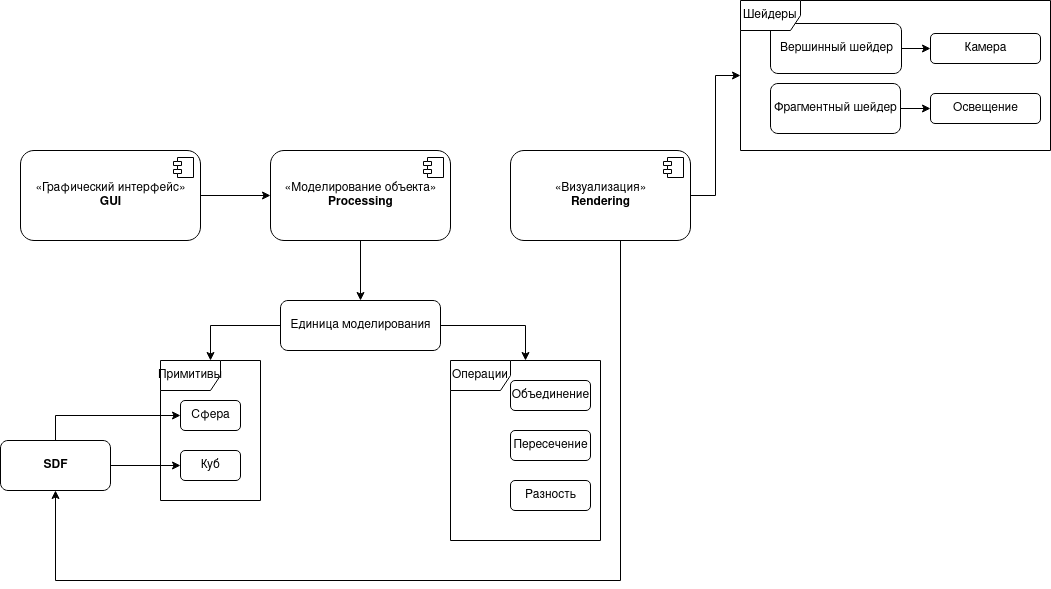
\includegraphics[scale=0.4]{inc/img/component_diagram}
  \caption{Схема приложения}
  \label{fig:app_scheme}
\end{figure}

На схеме представлено приложение, разделенное на функциональные части.
Пользователь может задать входные данные в графическом интерфейсе ($GUI$): примитивы, типы операций над ними,
положение камеры.
Выполнение отрисовки требует предварительного моделирования тела ($Processing$), которое описано рисунком \ref{fig:classes_diagram}, после
которого следует этап отрисовки, использующий шейдеры для установки положения камеры и выставления теней ($Rendering$).
% С помощью шейдеров модель закрашивается с учётом освещения.
% В результате полученное изображения отображается на экране и пользователь имеет возможность менять положение камеры.
% Весь процесс продолжается, пока пользователь не завершит выполнение.
% Для этапа моделирования были разработаны классы, которые представлены на рисунке \ref{fig:classes_diagram}.
% Помимо схемы, для проектируемого ПО приводится диаграмма классов моделирования тела ($Processing$ на схеме приложения).
% 
% \begin{figure}[H]
  % \centering
  % 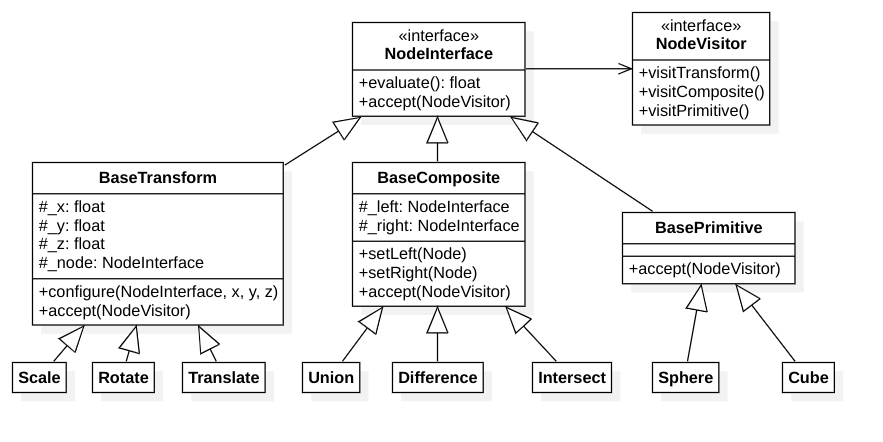
\includegraphics[scale=0.35]{inc/img/classes_diagram}
  % \caption{Диаграмма классов Processing}
  % \label{fig:classes_diagram}
% \end{figure}

% Для создания объектов в $CSG$ используется двоичное дерево.
% Данное дерево состоит из узлов, которые представлены в виде классов $Node$, которые являются реализацией интерфейса - 
% $BaseTransform$, $BaseComposite$, $BasePrimitive$.
% Класс $NodeInterface$ задаёт интерфейс для операций преобразования тел. 
% Все операции над моделью разделены на три группы: операции преобразования,
% операции композиции, операции создания примитивов. 

% Класс $BaseTransform$ предназначен для преобразования тела. Он содержит координаты 
% для перемещения/масштабирования/поворота модели. 
% Метод $configure$ конструирует экземпляр класса, принимая на вход модель - узел и координаты.  
% Класс $BaseComposite$ предназначен для конструирования модели с помощью $CSG$.  
% Он представляет собой дерево. Результатом обхода является модель. 
% Класс $BasePrimitive$ предназначен для создания примитивов, из которых происходит построение 
% модели.
% Класс $NodeVisitor$ реализует паттерн проектирования "Посетитель" и необходим для добавления
% нового функционала классам. В разрабатываемом ПО этот паттерн позволяет определить,
% какой класс представлен в $NodeInterface$, т.к его использование интерфейса подразумевает 
% абстрагирование от наследуемых реализаций. Обход происходит с помощью методов 
% $visitTransform$, $visitComposite$, $visitPrimitive$.  


\section{Вывод}
В данном разделе были рассмотренны методы и алгоритмы, необходимые для создания 
приложения. Была приведена схема приложения, представляющая архитектура проектируемого приложения.


%%% Local Variables:
%%% mode: latex
%%% TeX-master: "rpz"
%%% End:
